%%%%%%%%%%%%%%%%%%%%%%%%%%%%%%%%%%%%%%%%%%%%%%%%%%%%%%%%%%%%%%%%%%%%%%%%%%%%%%%%%%%%%%%%%
% This is a LaTeX template for Bachelor or Master theses at ZHAW, in accordance with the 
% guidelines provided here:
% https://www.zhaw.ch/en/lsfm/study/studiweb/master-ls/masters-thesis/
%
%
% This template is based on previous works by:
% Steve Gunn (http://users.ecs.soton.ac.uk/srg/softwaretools/document/templates/)
% Sunil Patel (http://www.sunilpatel.co.uk/thesis-template/)
% Matteo Delucchi (https://github.com/matteodelucchi/ZHAW_thesis-template)
%
% University specific changes were made by:
% Matteo Delucchi
% Norman Juchler
% 
% Template license:
% CC BY-NC-SA 3.0 (http://creativecommons.org/licenses/by-nc-sa/3.0/)
%%%%%%%%%%%%%%%%%%%%%%%%%%%%%%%%%%%%%%%%%%%%%%%%%%%%%%%%%%%%%%%%%%%%%%%%%%%%%%%%%%%%%%%%%

%----------------------------------------------------------------------------------------
% DOCUMENT SPECIFICATION
%----------------------------------------------------------------------------------------
\documentclass[
    11pt,                      % Default font size
    %oneside,                  % One-side binding. Default: Two-side binding / alternating margins
    english,                   % Language. Use ngerman for German (Neue Rechtschreibung)
    singlespacing,             % Spacing option: singlespacing, onehalfspacing or doublespacing
    %nolistspacing,            % Set spacing in lists to single
    %draft,                    % Enable draft mode: no pictures, no links, overfull hboxes indicated
    liststotoc,               % Include list of figures/tables/etc in the table of contents
    %toctotoc,                 % Include the main table of contents to the table of contents
    parskip,                  % Add vertical space between paragraphs
    %nohyperref,               % Disable links in the entire document
    % helveticafont,             % Uncomment to use Helvetica font
    headsepline,               % Show a horizontal line under the header
    %chapterinoneline,         % Place the chapter title and chapter number on one line
    consistentlayout,          % Have the same layout for special chapters: 
                               % declaration, abstract and acknowledgements
]{MastersDoctoralThesis}

% Uncomment the following lines to only include a subset of chapters.
% This is useful for long documents, as typesetting takes a bit of time
%\includeonly{
%    Front/titlepage,
%    Front/imprint,
%    Front/abstract,
%    %Front/declaration,
%    %Front/acknowledgements,
%    %Front/symbols,
%    Chapters/Chapter1,
%    %Chapters/Chapter2
%    }


%----------------------------------------------------------------------------------------
% PREAMBLE: PACKAGES AND CONFIGURATIONS
%----------------------------------------------------------------------------------------
% !TEX root = main.tex

%----------------------------
%   Fonts and characters
%----------------------------

% Support for special characters
\usepackage[utf8]{inputenc}    % Specify input encoding
\usepackage[T1]{fontenc}       % Specify font encoding
\usepackage{amssymb}       % Specify font encoding

% Set main fonts
% Fonts catalogue: https://tug.org/FontCatalogue/
\usepackage{mathpazo}          % Use the Palatino font by default
\usepackage{beramono}          % Override the monospace/typewriter font
\usepackage{caption}
\usepackage{subcaption}
\usepackage{multirow}
% ZHAW title font
% Try to load Helvetica Rounded Bold, and OpenType font.
% Loading OTF or system fonts is possible with XeLaTeX.
% If the document is compiled using pdfLaTeX, resort 
\usepackage{ifxetex}
\ifxetex
    \usepackage{fontspec}
    \newfontfamily\zhawtitlefont{Helvetica Rounded Bold}
\else
    \newcommand{\zhawtitlefont}{\scshape}
\fi

%\usepackage[scaled]{helvet}

%----------------------------
%   Environments
%----------------------------

\usepackage{caption}           % Customized caption
\usepackage{subcaption}        % Subfigure captions
\usepackage{makecell}          % Per-cell formatting in tables (\makecell)
\usepackage{pdfpages}          % Required to include PDF files/graphics (\includepdf)

\usepackage{todonotes}         % Introduces the command \todo
\setlength{\marginparwidth}{2.5cm} % Adjust this if the todo notes are out of margins

% Create boxes as follows:
% \begin{colorbox}{red}{2}
\usepackage{tcolorbox}
\newtcolorbox{textbox}[2]{
    arc=3pt,
    boxrule=#2pt,
    colback=#1!25!white,
    width=\textwidth,
    halign=left,
    valign=center,
    colframe=#1!75!black
}

%----------------------------
%   Colors
%----------------------------

% Set up colors
\usepackage{xcolor}
% ZHAW Blue: Pantone 2945 U / R0 G100 B166
\definecolor{zhawblue}{rgb}{0.00, 0.39, 0.65}
% Colors related to code listings
\definecolor{codegreen}{rgb}{0,0.6,0}
\definecolor{codegray}{rgb}{0.5,0.5,0.5}
\definecolor{codepurple}{rgb}{0.58,0,0.82}
\definecolor{codebackground}{rgb}{0.93,0.94,0.95}

%----------------------------
%   Code listings
%----------------------------

% Setup code listings
\usepackage{listings}
\lstdefinestyle{mystyle}{
    backgroundcolor=\color{codebackground},   
    commentstyle=\color{codegreen},
    keywordstyle=\color{magenta},
    numberstyle=\tiny\color{codegray},
    stringstyle=\color{codepurple},
    basicstyle=\ttfamily\footnotesize,
    breakatwhitespace=false,
    breaklines=true,
%    captionpos=b,
    keepspaces=true,
    numbers=left,
    numbersep=5pt,
    showspaces=false,
    showstringspaces=false,
    showtabs=false,
    tabsize=4
}
\lstset{style=mystyle}

% minted is an alternative code listing package. (See chapter 2)
% For it to run successfully, ensure the following:
% - the Python package Pygments. Install with the following command:
%       python -m pip install Pygments
% - pdflatex (or xelatex) is executed with the flag --shell-escape
%   If you are using a TEX editor, you can modify the typesetting 
%   command somewhere in the settings.
%\usepackage[outputdir=build]{minted}
%\usemintedstyle{xcode}
% For fancier coloring schemes, see here:
% https://tex.stackexchange.com/questions/585582
% One could also create an own style in Pygments
% https://pygments.org/docs/styles/#creating-own-styles

%----------------------------
%   References
%----------------------------

% Set up references
\usepackage[
    backend=biber,             % Use biber backend (an external tool)
    sorting=none,              % Enumerates the reference in order of their appearance
    style=numeric-comp         % Choose here your preferred citation style
]{biblatex}
\addbibresource{references.bib}   % The filename of the bibliography
\usepackage[autostyle=true]{csquotes} 
                               % Required to generate language-dependent quotes 
                               % in the bibliography

%----------------------------------------------------------------------------------------
%   MARGIN SETTINGS
%----------------------------------------------------------------------------------------

\geometry{
    paper=a4paper,      % Change to letterpaper for US letter
    inner=2.5cm,        % Inner margin
    outer=3.8cm,        % Outer margin
    top=1.5cm,          % Top margin
    bottom=1.5cm,       % Bottom margin
    bindingoffset=.5cm, % Binding offset
    %showframe,         % Show the type block of the page
}
\setlength{\parskip}{1em}
\usepackage{enumitem}          % Layout control for list environments (e.g, itemize)
%\setlist{noitemsep}           % Suppress extra spaces between items
%\setlist{nosep}               % Suppress spaces before/after list environments



%----------------------------------------------------------------------------------------
% THESIS INFORMATION: MODIFY THIS SECTION!
%----------------------------------------------------------------------------------------

% The information below is used in the following parts:
% - Title page
% - Imprint
% - Abstract / Zusammenfassung
% - Meta information of PDF

\thesistitle{Deep learning assisted X-ray photoelectron spectroscopy analysis}             % Thesis title,              command: \ttitle
\thesistype{Master Thesis}             % Type of thesis (e.g. Master Thesis) \ttype
\thesisdate{\today}                     % Date of submission                  \tdate
\keywords{XPS, x-ray, spectroscopy, photoelectron, deep learning}
                                        % Keywords for the thesis,            \keywordnames
\author{Kilian Koch}                  % Your name,                          \authorname
\degree{Master of Science ZFH}          % Degree name,                        \degreename
\studyprogram{Applied Computational Life Sciences, M.Sc.} 
                                        % Study program                       \studyprog
\studyprogramlink{https://www.zhaw.ch/en/lsfm/study/master/applied-computational-life-sciences/}
                                        % Link to study program               \studyproglink

\supervisorA{Dr. Martin Schüle}       % Name of supervisor 1,               \supnameA
\supervisorAmail{martin.schuele@zhaw.ch}         % Email address of supervisor 1,      \supmailA
\supervisorAweb{https://www.zhaw.ch/de/ueber-uns/person/scli/}  %            \supwebA
\supervisorAinfo{                       % Formatted info about supervisor 1:  \supinfoA
    \supnameA\\
    Zurich University of Applied Sciences\\
    Email: \href{mailto:\supmailA}{\supmailA}\\
    Web: \href{\supwebA}{Link}
}

% Keep empty if there is no supervisor 2: \supervisorB{}
\supervisorB{PD Dr. Andreas Borgschulte}              % Name of supervisor 2,               \supnameB
\supervisorBmail{andreas.borgschulte@empa.ch}       % Email address of supervisor 2,      \supmailB
\supervisorBweb{https://www.empa.ch/web/s502/research}                  % \supwebB
\supervisorBinfo{                       % Formatted info about supervisor 2:  \supinfoB
    \supnameB\\
    University of Zurich\\
    Email: \href{mailto:\supmailB}{\supmailB}\\
    Web: \href{\supwebB}{Link}
}

\university{Zurich University of Applied Sciences}
                                        % University name                     \univname
\universitygerman{Zürcher Hochschule für Angewandte Wissenschaften}
                                        % University, in German               \univnameger
\department{Life Sciences and Facility Management} 
                                        % Department,                         \deptname
\institute{Institute of Computational Life Sciences} 
                                        % Institute,                          \instname
\group{Center of Computational Health} 
                                        % Research group                      \groupname

% Links
\universitylink      {https://www.zhaw.ch/en/university/}                   % \univlink
\universitylinkgerman{https://www.zhaw.ch/de/university/}                   % \univlinkger
\departmentlink      {https://www.zhaw.ch/de/lsfm/}                         % \deptlink
\institutelink       {https://www.zhaw.ch/en/lsfm/institutes-centres/icls/} % \instlink
\grouplink           {https://www.zhaw.ch/en/lsfm/institutes-centres/icls/computational-health/} % \grplink



\AtBeginDocument{
\hypersetup{pdftitle=\ttitle} % Set the PDF's title to your title
\hypersetup{pdfauthor=\authorname} % Set the PDF's author to your name
\hypersetup{pdfkeywords=\keywordnames} % Set the PDF's keywords to your keywords
}

\begin{document}
\frontmatter                  % Roman page numbering for the pre-content pages
\pagestyle{plain}             % Default to the plain heading style until the thesis style 
                              % is called for the body content


%----------------------------------------------------------------------------------------
% TITLE PAGE AND IMPRINT
%----------------------------------------------------------------------------------------
\include{Front/titlepage}
\let\cleardoublepage\clearpage
\include{Front/imprint}


%----------------------------------------------------------------------------------------
% DECLARATION
%----------------------------------------------------------------------------------------
% Comment out this section if the declaration of originality from ZHAW is used.
% !TEX root = ../main.tex

%----------------------------------------------------------------------------------------
% DECLARATION OF ORIGINALITY
%----------------------------------------------------------------------------------------

\begin{declaration}
\addchaptertocentry{\authorshipname} % Add the declaration to the table of contents

\begin{textbox}{red}{2}
REMOVE THIS SECTION IF THE \href{https://www.zhaw.ch/en/lsfm/study/studiweb/master-ls/masters-thesis/}{ORIGINAL COPY OF THE ZHAW DECLARATION OF ORIGINALITY} IS USED IN THE APPENDIX.
\end{textbox}
\vspace{1cm}

\noindent I, \authorname, declare that this thesis titled, \enquote{\ttitle} and the work presented in it are my own. I confirm that:

\begin{itemize} 
\item This work was done wholly or mainly while in candidature for a research degree at the \univname.
\item Where any part of this thesis has previously been submitted for a degree or any other qualification at this university or any other institution, this has been clearly stated.
\item Where I have consulted the published work of others, this is always clearly attributed.
\item Where I have quoted from the work of others, the source is always given. With the exception of such quotations, this thesis is entirely my own work.
\item I have acknowledged all main sources of help.
\item Where the thesis is based on work done by myself jointly with others, 
I have made clear exactly what was done by others and what I have contributed myself.\\
\end{itemize}
\vspace{1cm}

\noindent Signed:\\
\rule[0.5em]{25em}{0.5pt} % This prints a line for the signature
 
\noindent Date:\\
\rule[0.5em]{25em}{0.5pt} % This prints a line to write the date
\end{declaration}

\cleardoublepage


%----------------------------------------------------------------------------------------
% ABSTRACT
%----------------------------------------------------------------------------------------
% !TEX root = ../main.tex

%----------------------------------------------------------------------------------------
% ABSTRACT PAGE
%----------------------------------------------------------------------------------------
\begin{abstract}
\addchaptertocentry{\abstractname} % Add the abstract to the table of contents
Surface analysis for the determination of chemical composition of a solid palys an important role in material sciences. X-ray photoelectron spectroscopy is widely applied for such structural analysis, giving information beyond the outermost surface, as it probes deeper to approximately 10 nanometers depth. Analysis of the spectrum to model the solid under investigation is complex, as many effects complain the inference, such as inelastic and elastic scattering and sample contamination. This work applies deep learning models to three main problems; qualitative identification, quantitative identification and depth profiling.
To overcome the lack of available labelled XPS data, a simulation software was used to obtain >300k XPS spectra as training data. Four different models architectures were applied to the main problems; convolutional neural network (CNN), convolutional dct-informed neural network (CNN-DCT), Residual convolutional block attention model (CBAM) and Vision Transformer (ViT). 
\end{abstract}


%----------------------------------------------------------------------------------------
% German ABSTRACT PAGE
%----------------------------------------------------------------------------------------
\begin{extraAbstract}
\addchaptertocentry{\extraabstractname} % Add the abstract to the table of contents

Die Zusammenfassung entspricht einer Miniaturversion des gesamten Dokuments. Gliedere sie ähnlich: Beginne mit dem Kontext und der Motivation für das Projekt, einer kurzen Beschreibung der Methode und der verfügbaren Daten, Ihren Ergebnissen und den Schlussfolgerungen. Beschränke dich auf eine Seite!    
\end{extraAbstract}



%----------------------------------------------------------------------------------------
% ACKNOWLEDGEMENTS
%----------------------------------------------------------------------------------------
\include{Front/acknowledgements}


%----------------------------------------------------------------------------------------
% LIST OF CONTENTS/FIGURES/TABLES PAGES
%----------------------------------------------------------------------------------------
% Comment out if any of the following is not needed:
\tableofcontents  % Add main table of contents
%\listoffigures    % Add list of figures
%\listoftables     % Add list of tables


%----------------------------------------------------------------------------------------
% ABBREVIATIONS / SYMBOLS
%----------------------------------------------------------------------------------------
\include{Front/symbols}


%----------------------------------------------------------------------------------------
% DEDICATION
%----------------------------------------------------------------------------------------
\dedicatory{For/Dedicated to/To my\ldots} 


%----------------------------------------------------------------------------------------
% THESIS CONTENT - CHAPTERS
%----------------------------------------------------------------------------------------
\mainmatter % Begin numeric (1,2,3...) page numbering
\pagestyle{thesis} % Return the page headers back to the "thesis" style

% Include the chapters of the thesis as separate files from the Chapters folder
% Uncomment the lines as you write the chapters

% Indicate the main file. Must go at the beginning of the file.
% !TEX root = ../main.tex

%----------------------------------------------------------------------------------------
% CHAPTER 1
%----------------------------------------------------------------------------------------



\chapter{Introduction to \LaTeX} % Main chapter title
\label{Chapter1} % For referencing the chapter elsewhere, use \ref{Chapter1} 

%----------------------------------------------------------------------------------------

% Define some commands to keep the formatting separated from the content
% Placing such commands in the preamble is a good idea.
\newcommand{\keyword}[1]{\textbf{#1}}
\newcommand{\tabhead}[1]{\textbf{#1}}
\newcommand{\code}[1]{\texttt{#1}}
\newcommand{\file}[1]{\texttt{\bfseries#1}}
\newcommand{\option}[1]{\texttt{\itshape#1}}

%----------------------------------------------------------------------------------------

\section{Welcome and Thank You}
Welcome to this \LaTeX{} Thesis Template, a beautiful and easy to use template for writing a thesis using the \LaTeX{} typesetting system.

If you are writing a thesis (or will be in the future) and its subject is technical or mathematical (though it doesn't have to be), then creating it in \LaTeX{} is highly recommended as a way to make sure you can just get down to the essential writing without having to worry over formatting or wasting time arguing with your word processor.

\LaTeX{} is easily able to professionally typeset documents that run to hundreds or thousands of pages long. With simple mark-up commands, it automatically sets out the table of contents, margins, page headers and footers and keeps the formatting consistent and beautiful. One of its main strengths is the way it can easily typeset mathematics, even \emph{heavy} mathematics. Even if those equations are the most horribly twisted and most difficult mathematical problems that can only be solved on a super-computer, you can at least count on \LaTeX{} to make them look stunning.

%----------------------------------------------------------------------------------------

\section{Learning \LaTeX{}}

\LaTeX{} is not a \textsc{wysiwyg} (What You See is What You Get) program, unlike word processors such as Microsoft Word or Apple's Pages. Instead, a document written for \LaTeX{} is actually a simple, plain text file that contains \emph{no formatting}. You tell \LaTeX{} how you want the formatting in the finished document by writing in simple commands amongst the text, for example, if I want to use \emph{italic text for emphasis}, I write the \verb|\emph{text}| command and put the text I want in italics in between the curly braces. This means that \LaTeX{} is a \enquote{mark-up} language, very much like HTML.

\subsection{A (not so short) Introduction to \LaTeX{}}

If you are new to \LaTeX{}, there is a very good eBook -- freely available online as a PDF file -- called, \enquote{The Not So Short Introduction to \LaTeX{}}. The book's title is typically shortened to just \emph{lshort}. You can download the latest version (as it is occasionally updated) from here:
\url{http://www.ctan.org/tex-archive/info/lshort/english/lshort.pdf}

It is also available in several other languages. Find yours from the list on this page: \url{http://www.ctan.org/tex-archive/info/lshort/}

It is recommended to take a little time out to learn how to use \LaTeX{} by creating several, small `test' documents, or having a close look at several templates on:\\ 
\url{http://www.LaTeXTemplates.com}\\ 
Making the effort now means you're not stuck learning the system when what you \emph{really} need to be doing is writing your thesis.

\subsection{A Short Math Guide for \LaTeX{}}

If you are writing a technical or mathematical thesis, then you may want to read the document by the AMS (American Mathematical Society) called, \enquote{A Short Math Guide for \LaTeX{}}. It can be found online:

\url{http://www.ams.org/tex/amslatex.html} $\rightarrow$ \enquote{Additional Documentation}\\
\url{https://mirror.foobar.to/CTAN/info/short-math-guide/}

\subsection{Common \LaTeX{} Math Symbols}
There are a multitude of mathematical symbols available for \LaTeX{} and it would take a great effort to learn the commands for them all. The most common ones you are likely to use are shown on this page:
\url{http://www.sunilpatel.co.uk/latex-type/latex-math-symbols/}

You can use this page as a reference or crib sheet, the symbols are rendered as large, high quality images so you can quickly find the \LaTeX{} command for the symbol you need.

\subsection{\LaTeX{} on a Mac}
 
The \LaTeX{} distribution is available for many systems including Windows, Linux and Mac OS X. The package for OS X is called MacTeX and it contains all the applications you need -- bundled together and pre-customized -- for a fully working \LaTeX{} environment and work flow.
 
MacTeX includes a custom dedicated \LaTeX{} editor called TeXShop for writing your `\file{.tex}' files and BibDesk: a program to manage your references and create your bibliography section just as easily as managing songs and creating playlists in iTunes.

%----------------------------------------------------------------------------------------

\section{Getting Started with this Template}

If you are familiar with \LaTeX{}, then you should explore the directory structure of the template and then proceed to place your own information into the \emph{THESIS INFORMATION} block of the \file{main.tex} file. You can then modify the rest of this file to your unique specifications based on your degree/university. Section \ref{FillingFile} on page \pageref{FillingFile} will help you do this. Make sure you also read section \ref{ThesisConventions} about thesis conventions to get the most out of this template.

If you are new to \LaTeX{} it is recommended that you carry on reading through the rest of the information in this document.

Before you begin using this template you should ensure that its style complies with the thesis style guidelines imposed by your institution. In most cases this template style and layout will be suitable. If it is not, it may only require a small change to bring the template in line with your institution's recommendations. These modifications will need to be done on the \file{MastersDoctoralThesis.cls} file.

\subsection{About this Template}

This \LaTeX{} Thesis Template is originally based and created around a \LaTeX{} style file created by Steve R.\ Gunn from the University of Southampton (UK), department of Electronics and Computer Science. You can find his original thesis style file at his site, here:
\url{http://www.ecs.soton.ac.uk/~srg/softwaretools/document/templates/}

Steve's \file{ecsthesis.cls} was then taken by Sunil Patel who modified it by creating a skeleton framework and folder structure to place the thesis files in. The resulting template can be found on Sunil's site here:
\url{http://www.sunilpatel.co.uk/thesis-template}


Sunil's template was made available through \url{http://www.LaTeXTemplates.com}, where it was modified many times based on user requests and questions. Version 2.0 and onwards of this template represents a major modification to Sunil's template and is, in fact, hardly recognisable. The work to make version 2.0 possible was carried out by \href{mailto:vel@latextemplates.com}{Vel} and Johannes Böttcher.

Based on Sunil's Version 2.0, Matteo updated the template and incorporated ZHAW University thesis guidelines.

%----------------------------------------------------------------------------------------

\section{What this Template Includes}

\subsection{Folders}

This template comes as a single zip file that expands out to several files and folders. The folder names are mostly self-explanatory:

\keyword{Appendices} -- this is the folder where you put the appendices. Each appendix should go into its own separate \file{.tex} file. An example and template are included in the directory.

\keyword{Chapters} -- this is the folder where you put the thesis chapters. A thesis usually has about six chapters, though there is no hard rule on this. Each chapter should go in its own separate \file{.tex} file and they can be split as:
\begin{itemize}
\item Chapter 1: Introduction to the thesis topic
\item Chapter 2: Background information and theory
\item Chapter 3: (Laboratory) experimental setup
\item Chapter 4: Details of experiment 1
\item Chapter 5: Details of experiment 2
\item Chapter 6: Discussion of the experimental results
\item Chapter 7: Conclusion and future directions
\end{itemize}
This chapter layout is specialised for the experimental sciences, your discipline may be different.

\keyword{Figures} -- this folder contains all figures for the thesis. These are the final images that will go into the thesis document.

\subsection{Files}

Included are also several files, most of them are plain text and you can see their contents in a text editor. After initial compilation, you will see that more auxiliary files are created by \LaTeX{} or BibTeX and which you don't need to delete or worry about:

\keyword{example.bib} -- this is an important file that contains all the bibliographic information and references that you will be citing in the thesis for use with BibTeX. You can write it manually, but there are reference manager programs available that will create and manage it for you. Bibliographies in \LaTeX{} are a large subject and you may need to read about BibTeX before starting with this. Many modern reference managers will allow you to export your references in BibTeX format which greatly eases the amount of work you have to do.

\keyword{MastersDoctoralThesis.cls} -- this is an important file. It is the class file that tells \LaTeX{} how to format the thesis. 

\keyword{main.pdf} -- this is your beautifully typeset thesis (in the PDF file format) created by \LaTeX{}. It is supplied in the PDF with the template and after you compile the template you should get an identical version.

\keyword{main.tex} -- this is an important file. This is the file that you tell \LaTeX{} to compile to produce your thesis as a PDF file. It contains the framework and constructs that tell \LaTeX{} how to layout the thesis. It is heavily commented so you can read exactly what each line of code does and why it is there. After you put your own information into the \emph{THESIS INFORMATION} block -- you have now started your thesis!

Files that are \emph{not} included, but are created by \LaTeX{} as auxiliary files include:

\keyword{main.aux} -- this is an auxiliary file generated by \LaTeX{}, if it is deleted \LaTeX{} simply regenerates it when you run the main \file{.tex} file.

\keyword{main.bbl} -- this is an auxiliary file generated by BibTeX, if it is deleted, BibTeX simply regenerates it when you run the \file{main.aux} file. Whereas the \file{.bib} file contains all the references you have, this \file{.bbl} file contains the references you have actually cited in the thesis and is used to build the bibliography section of the thesis.

\keyword{main.blg} -- this is an auxiliary file generated by BibTeX, if it is deleted BibTeX simply regenerates it when you run the main \file{.aux} file.

\keyword{main.lof} -- this is an auxiliary file generated by \LaTeX{}, if it is deleted \LaTeX{} simply regenerates it when you run the main \file{.tex} file. It tells \LaTeX{} how to build the \emph{List of Figures} section.

\keyword{main.log} -- this is an auxiliary file generated by \LaTeX{}, if it is deleted \LaTeX{} simply regenerates it when you run the main \file{.tex} file. It contains messages from \LaTeX{}, if you receive errors and warnings from \LaTeX{}, they will be in this \file{.log} file.

\keyword{main.lot} -- this is an auxiliary file generated by \LaTeX{}, if it is deleted \LaTeX{} simply regenerates it when you run the main \file{.tex} file. It tells \LaTeX{} how to build the \emph{List of Tables} section.

\keyword{main.out} -- this is an auxiliary file generated by \LaTeX{}, if it is deleted \LaTeX{} simply regenerates it when you run the main \file{.tex} file.

So from this long list, only the files with the \file{.bib}, \file{.cls} and \file{.tex} extensions are the most important ones. The other auxiliary files can be ignored or deleted as \LaTeX{} and BibTeX will regenerate them.

%----------------------------------------------------------------------------------------

\section{Filling in Your Information in the \file{main.tex} File}\label{FillingFile}

You will need to personalise the thesis template and make it your own by filling in your own information. This is done by editing the \file{main.tex} file in a text editor or your favourite LaTeX environment.

Open the file and scroll down to the third large block titled \emph{THESIS INFORMATION} where you can see the entries for \emph{University Name}, \emph{Department Name}, etc \ldots

Fill out the information about yourself, your group and institution. You can also insert web links, if you do, make sure you use the full URL, including the \code{http://} for this. If you don't want these to be linked, simply remove the \verb|\href{url}{name}| and only leave the name.

When you have done this, save the file and recompile \code{main.tex}. All the information you filled in should now be in the PDF, complete with web links. You can now begin your thesis proper!

%----------------------------------------------------------------------------------------

\section{The \code{main.tex} File Explained}

The \file{main.tex} file contains the structure of the thesis. There are plenty of written comments that explain what pages, sections and formatting the \LaTeX{} code is creating. Each major document element is divided into commented blocks with titles in all capitals to make it obvious what the following bit of code is doing. Initially there seems to be a lot of \LaTeX{} code, but this is all formatting, and it has all been taken care of so you don't have to do it.

Begin by checking that your information on the title page is correct. For the thesis declaration, your institution may insist on something different than the text given. If this is the case, just replace what you see with what is required in the \emph{DECLARATION PAGE} block.

Then comes a page which contains a funny quote. You can put your own, or quote your favourite scientist, author, person, and so on. Make sure to put the name of the person who you took the quote from.

Following this is the abstract page which summarises your work in a condensed way and can almost be used as a standalone document to describe what you have done. The text you write will cause the heading to move up so don't worry about running out of space.

Next come the acknowledgements. On this page, write about all the people who you wish to thank (not forgetting parents, partners and your advisor/supervisor).

The contents pages, list of figures and tables are all taken care of for you and do not need to be manually created or edited. The next set of pages are more likely to be optional and can be deleted since they are for a more technical thesis: insert a list of abbreviations you have used in the thesis, then a list of the physical constants and numbers you refer to and finally, a list of mathematical symbols used in any formulae. Making the effort to fill these tables means the reader has a one-stop place to refer to instead of searching the internet and references to try and find out what you meant by certain abbreviations or symbols.

The list of symbols is split into the Roman and Greek alphabets. Whereas the abbreviations and symbols ought to be listed in alphabetical order (and this is \emph{not} done automatically for you) the list of physical constants should be grouped into similar themes.

The next page contains a one line dedication. Who will you dedicate your thesis to?

Finally, there is the block where the chapters are included. Uncomment the lines (delete the \code{\%} character) as you write the chapters. Each chapter should be written in its own file and put into the \emph{Chapters} folder and named \file{Chapter1}, \file{Chapter2}, etc\ldots Similarly for the appendices, uncomment the lines as you need them. Each appendix should go into its own file and placed in the \emph{Appendices} folder.

After the preamble, chapters and appendices finally comes the bibliography. The bibliography style (called \option{authoryear}) is used for the bibliography and is a fully featured style that will even include links to where the referenced paper can be found online. Do not underestimate how grateful your reader will be to find that a reference to a paper is just a click away. Of course, this relies on you putting the URL information into the BibTeX file in the first place.

%----------------------------------------------------------------------------------------

\section{Thesis Features and Conventions}\label{ThesisConventions}

To get the best out of this template, there are a few conventions that you may want to follow.

One of the most important (and most difficult) things to keep track of in such a long document as a thesis is consistency. Using certain conventions and ways of doing things (such as using a Todo list) makes the job easier. Of course, all of these are optional and you can adopt your own method.

\subsection{Printing Format}

This thesis template is designed for double sided printing (i.e. content on the front and back of pages) as most theses are printed and bound this way. To switch to one sided printing, uncomment the \option{oneside} option of the \code{documentclass} command at the top of the \file{main.tex} file. You may then wish to adjust the margins to suit specifications from your institution.

The headers for the pages contain the page number on the outer side (so it is easy to flick through to the page you want) and the chapter name on the inner side.

The text is set to 11 point by default with single line spacing, again, you can tune the text size and spacing should you want or need to using the options at the very start of \file{main.tex}. The spacing can be changed similarly by replacing the \option{singlespacing} with \option{onehalfspacing} or \option{doublespacing}.

\subsection{Using US Letter Paper}

The paper size used in the template is A4, which is the standard size in Europe. If you are using this thesis template elsewhere and particularly in the United States, then you may have to change the A4 paper size to the US Letter size. This can be done in the margins settings section in \file{main.tex}.

Due to the differences in the paper size, the resulting margins may be different to what you like or require (as it is common for institutions to dictate certain margin sizes). If this is the case, then the margin sizes can be tweaked by modifying the values in the same block as where you set the paper size. Now your document should be set up for US Letter paper size with suitable margins.

\subsection{References}

The \code{biblatex} package is used to format the bibliography and inserts references such as this one \parencite{Reference1}. 
The inline citation style can be changed to e.g. authoryear in the \file{main.tex} file. 
\href{https://www.overleaf.com/learn/latex/Biblatex_citation_styles}{This documentation} lists and explains different standard citation styles.
The options used in the \file{main.tex} file mean that the in-text citations of references are formatted with the author(s) listed with the date of the publication. Multiple references are separated by semicolons (e.g. \parencite{Reference2, Reference1}) and references with more than three authors only show the first author with \emph{et al.} indicating there are more authors (e.g. \parencite{Reference3}). This is done automatically for you. To see how you use references, have a look at the \file{Chapter1.tex} source file. Many reference managers allow you to simply drag the reference into the document as you type.

Scientific references should come \emph{before} the punctuation mark if there is one (such as a comma or period). The same goes for footnotes\footnote{Such as this footnote, here down at the bottom of the page.}. You can change this but the most important thing is to keep the convention consistent throughout the thesis. Footnotes themselves should be full, descriptive sentences (beginning with a capital letter and ending with a full stop). The APA6 states: \enquote{Footnote numbers should be superscripted, [...], following any punctuation mark except a dash.} The Chicago manual of style states: \enquote{A note number should be placed at the end of a sentence or clause. The number follows any punctuation mark except the dash, which it precedes. It follows a closing parenthesis.}

The bibliography is typeset with references listed in alphabetical order by the first author's last name. This is similar to the APA referencing style. To see how \LaTeX{} typesets the bibliography, have a look at the very end of this document (or just click on the reference number links in in-text citations).

\subsubsection{A Note on bibtex}

The bibtex backend used in the template by default does not correctly handle unicode character encoding (i.e. "international" characters). You may see a warning about this in the compilation log and, if your references contain unicode characters, they may not show up correctly or at all. The solution to this is to use the biber backend instead of the outdated bibtex backend. This is done by finding this in \file{main.tex}: \option{backend=bibtex} and changing it to \option{backend=biber}. You will then need to delete all auxiliary BibTeX files and navigate to the template directory in your terminal (command prompt). Once there, simply type \code{biber main} and biber will compile your bibliography. You can then compile \file{main.tex} as normal and your bibliography will be updated. An alternative is to set up your LaTeX editor to compile with biber instead of bibtex, see \href{http://tex.stackexchange.com/questions/154751/biblatex-with-biber-configuring-my-editor-to-avoid-undefined-citations/}{here} for how to do this for various editors.

\subsection{Tables}

Tables are an important way of displaying your results, below is an example table which was generated with this code:

{\small
    \begin{verbatim}
    \begin{table}
    \caption{The effects of treatments X and Y 
            on the four groups studied.}
    \label{tab:treatments}
    \centering
    \begin{tabular}{l l l}
    \toprule
    \tabhead{Groups} & \tabhead{Treatment X} & \tabhead{Treatment Y} \\
    \midrule
    1 & 0.2 & 0.8\\
    2 & 0.17 & 0.7\\
    3 & 0.24 & 0.75\\
    4 & 0.68 & 0.3\\
    \bottomrule\\
    \end{tabular}
    \end{table}
    \end{verbatim}
}

\begin{table}
\caption{The effects of treatments X and Y on the four groups studied.}
\label{tab:treatments}
\centering
\begin{tabular}{l l l}
\toprule
\tabhead{Groups} & \tabhead{Treatment X} & \tabhead{Treatment Y} \\
\midrule
1 & 0.2 & 0.8\\
2 & 0.17 & 0.7\\
3 & 0.24 & 0.75\\
4 & 0.68 & 0.3\\
\bottomrule\\
\end{tabular}
\end{table}

You can reference tables with \verb|\ref{<label>}| where the label is defined within the table environment. See \file{Chapter1.tex} for an example of the label and citation (e.g. Table~\ref{tab:treatments}).

\subsection{Figures}

There will hopefully be many figures in your thesis (that should be placed in the \emph{Figures} folder). The way to insert figures into your thesis is to use a code template like this:
\begin{verbatim}
\begin{figure}
\centering

\includegraphics{Figures/Electron}
\decoRule
\caption[An Electron]{An electron (artist's impression).}
\label{fig:Electron}
\end{figure}
\end{verbatim}
Also look in the source file. Putting this code into the source file produces the picture of the electron that you can see in the figure below.

\begin{figure}[th]
\centering

\includegraphics{Figures/Electron}
\decoRule
\caption[An Electron]{An electron (artist's impression).}
\label{fig:Electron}
\end{figure}

Sometimes figures don't always appear where you write them in the source. The placement depends on how much space there is on the page for the figure. Sometimes there is not enough room to fit a figure directly where it should go (in relation to the text) and so \LaTeX{} puts it at the top of the next page. Positioning figures is the job of \LaTeX{} and so you should only worry about making them look good!

Figures usually should have captions just in case you need to refer to them (such as in Figure~\ref{fig:Electron}). The \verb|\caption| command contains two parts, the first part, inside the square brackets is the title that will appear in the \emph{List of Figures}, and so should be short. The second part in the curly brackets should contain the longer and more descriptive caption text.

The \verb|\decoRule| command is optional and simply puts an aesthetic horizontal line below the image. If you do this for one image, do it for all of them.

\LaTeX{} is capable of using images in pdf, jpg and png format.

\subsection{Typesetting mathematics}

If your thesis is going to contain heavy mathematical content, be sure that \LaTeX{} will make it look beautiful, even though it won't be able to solve the equations for you.

The \enquote{Not So Short Introduction to \LaTeX} (available on \href{http://www.ctan.org/tex-archive/info/lshort/english/lshort.pdf}{CTAN}) should tell you everything you need to know for most cases of typesetting mathematics. If you need more information, a much more thorough mathematical guide is available from the AMS called, \enquote{A Short Math Guide to \LaTeX} and can be downloaded from:
\url{ftp://ftp.ams.org/pub/tex/doc/amsmath/short-math-guide.pdf}

There are many different \LaTeX{} symbols to remember, luckily you can find the most common symbols in \href{http://ctan.org/pkg/comprehensive}{The Comprehensive \LaTeX~Symbol List}.

You can write an equation, which is automatically given an equation number by \LaTeX{} like this:
\begin{verbatim}
\begin{equation}
E = mc^{2}
\label{eqn:Einstein}
\end{equation}
\end{verbatim}

This will produce Einstein's famous energy-matter equivalence equation:
\begin{equation}
E = mc^{2}
\label{eqn:Einstein}
\end{equation}

All equations you write (which are not in the middle of paragraph text) are automatically given equation numbers by \LaTeX{}. If you don't want a particular equation numbered, use the unnumbered form:
\begin{verbatim}
\[ a^{2}=4 \]
\end{verbatim}

%----------------------------------------------------------------------------------------

\section{Sectioning and Subsectioning}

You should break your thesis up into nice, bite-sized sections and subsections. \LaTeX{} automatically builds a table of contents by looking at all \verb|\chapter{}|, \verb|\section{}|  and \verb|\subsection{}| commands you write in the source.

The Table of Contents should only list the sections to three (3) levels. A \verb|chapter{}| is level zero (0). A \verb|\section{}| is level one (1) and so a \verb|\subsection{}| is level two (2). In your thesis it is likely that you will even use a \verb|subsubsection{}|, which is level three (3). The depth to which the Table of Contents is formatted is set within \file{MastersDoctoralThesis.cls}. If you need this changed, you can do it in \file{main.tex}.

%----------------------------------------------------------------------------------------

\section{In Closing}

You have reached the end of this mini-guide. You can now rename or overwrite this pdf file and begin writing your own \file{Chapter1.tex} and the rest of your thesis. The easy work of setting up the structure and framework has been taken care of for you. It's now your job to fill it out!

Good luck and have lots of fun!

\begin{flushright}
Guide written by ---\\
Sunil Patel: \href{http://www.sunilpatel.co.uk}{www.sunilpatel.co.uk}\\
Vel: \href{http://www.LaTeXTemplates.com}{LaTeXTemplates.com}
\end{flushright}

\include{Chapters/Chapter2} 
%\include{Chapters/Chapter3}
%\include{Chapters/Chapter4} 
%\include{Chapters/Chapter5} 


%----------------------------------------------------------------------------------------
% THESIS CONTENT - APPENDICES
%----------------------------------------------------------------------------------------
\appendix % Cue to tell LaTeX that the following "chapters" are Appendices

% Include the appendices of the thesis as separate files from the Appendices folder
% Uncomment the lines as you write the Appendices
% !TEX root = ../main.tex

%----------------------------------------------------------------------------------------
% APPENDIX A
%----------------------------------------------------------------------------------------

\chapter{Code} % Main appendix title

\label{AppendixA} % For referencing this appendix elsewhere, use \ref{AppendixA}

\section{Modules}

\subsection{Base module}
\label{code:base}
\lstinputlisting[language=Python]{Code/modules/base.py}

\subsection{Functions module}
\label{code:functions}
\lstinputlisting[language=Python]{Code/modules/functions_tf.py}

\subsection{Preprocessing module}
\label{preprocessing}
\lstinputlisting[language=Python]{Code/modules/preprocess.py}

\subsection{Prediction module}
\label{code:base}
\lstinputlisting[language=Python]{Code/modules/predict.py}

\subsection{Sessa Simulation module}
\label{Sessa_Module}
\lstinputlisting[language=Python]{Code/modules/sessa_py.py}



\section{Notebooks}

\subsection{NIST Chemical Shift Database Webscraper}
\label{NIST_WebScraper}
\lstinputlisting[language=Python]{Code/modules/req_async.py}

\subsection{XPSLibrary Webscraper}
\label{xpslibrary_webscraper}
\subsubsection*{Grab folders from XPSSurfA}\label{grab-folders-from-xpssurfa}

\begin{lstlisting}[language=Python]
from bs4 import BeautifulSoup
import os
import requests
import urllib.request
import os
\end{lstlisting}

\begin{lstlisting}[language=Python]
number = 1
URL = f'https://cmsshub.latrobe.edu.au/xpsdatabase/xpsrecords/download_data_files/{number}'
req = requests.get(URL)
soup = BeautifulSoup(open('../../data/test_data/XPSSurfA/view-source_https___cmsshub.latrobe.edu.au_xpsdatabase_xpsrecords.html'),
                            'html.parser')
numbers = [int(p.get('href').split('/')[-1]) 
           for p in soup.findAll(class_="html-attribute-value html-external-link") 
           if 'view' in p.get('href')]
\end{lstlisting}

\begin{lstlisting}[language=Python]
for number in numbers:
    print(number)
    if os.path.isfile(f'../../data/test_data/XPSSurfA/{number}.zip'):
        print('already downloaded')
        continue
    URL = f'https://cmsshub.latrobe.edu.au/xpsdatabase/xpsrecords/download_data_files/{number}'
    file_name  = f'../../data/test_data/XPSSurfA/{number}.zip'
    # Download the file from `url` and save it locally under `file_name`:
    with urllib.request.urlopen(URL) as response, open(file_name, 'wb') as out_file:
        data = response.read() # a `bytes` object
        out_file.write(data)
\end{lstlisting}

\subsubsection*{Unzip all downloaded files from
XPSSurfA}\label{unzip-all-downloaded-files-from-xpslibrary.com}

\begin{lstlisting}[language=Python]
import os
import zipfile

root_folder = '../../data/test_data/XPSSurfA'

# add //? before path if the path is too long otherwise it will throw an error

def extract_zip_files(root_folder):
    for foldername, subfolders, filenames in os.walk(root_folder):
        for filename in filenames:
            if filename.endswith('.zip'):
                zip_file_path = os.path.join(foldername, filename)
                print(os.path.join(foldername, os.path.splitext(filename)[0]))
                with zipfile.ZipFile(zip_file_path, 'r') as zip_ref:
                    zip_ref.extractall(os.path.join(foldername, os.path.splitext(filename)[0]))
\end{lstlisting}

\begin{lstlisting}[language=Python]
extract_zip_files(root_folder)
\end{lstlisting}

\subsubsection*{Check files from XPSSurfA}\label{check-files-from-xpssurfa}

\begin{lstlisting}[language=Python]
files = []
for foldername, subfolders, filenames in os.walk(root_folder):
    # check if there is a *.vms file in the folder
    # print(foldername)
    if any([filename.endswith('.vms') for filename in filenames]):
        # print('yes')
        files.append(([foldername + '\\' +filename for filename in filenames if filename.endswith('.vms')][0]))
\end{lstlisting}

\begin{lstlisting}[language=Python]
len(files) # we have 121 test files
\end{lstlisting}

\begin{lstlisting}
121
\end{lstlisting}

\begin{lstlisting}[language=Python]
files = [f for f in files if len(f.split('_')) > 2 and len(f.split('_')[-1]) < 15 and not 'Cali' in f]
\end{lstlisting}

\begin{lstlisting}[language=Python]
files
\end{lstlisting}

\begin{lstlisting}
['../../data/test_data/XPSSurfA\\10\\Fe_Fe.vms',
 '../../data/test_data/XPSSurfA\\13\\Ar_Ar.vms',
 '../../data/test_data/XPSSurfA\\149\\Cu_Cu_Ultra.vms',
 '../../data/test_data/XPSSurfA\\15\\Mg_Mg.vms',
 '../../data/test_data/XPSSurfA\\150\\Ag_Ag_Ultra.vms',
 '../../data/test_data/XPSSurfA\\151\\Au_Au_Ultra.vms',
 '../../data/test_data/XPSSurfA\\154\\Nb_Nb.vms',
 '../../data/test_data/XPSSurfA\\16\\Ni_Ni.vms',
 '../../data/test_data/XPSSurfA\\17\\Mo_Mo.vms',
 '../../data/test_data/XPSSurfA\\18\\Ta_Ta.vms',
 '../../data/test_data/XPSSurfA\\2\\Au_Au.vms',
 '../../data/test_data/XPSSurfA\\20\\Al_Al.vms',
 '../../data/test_data/XPSSurfA\\22\\Si_Si.vms',
 '../../data/test_data/XPSSurfA\\3\\Ag_Ag.vms',
 '../../data/test_data/XPSSurfA\\4\\Pt_Pt.vms',
 '../../data/test_data/XPSSurfA\\5\\Cu_Cu.vms',
 '../../data/test_data/XPSSurfA\\7\\W_W.vms',
 '../../data/test_data/XPSSurfA\\9\\In_In.vms']
\end{lstlisting}


\subsection{Sessa Simulation Notebook}
\label{xpslibrary_webscraper}
\hypertarget{define-directories}{%
\section*{Define directories}\label{define-directories}}

\begin{lstlisting}[language=Python]
from sessa_py import Experiment, Layer
import os
import numpy as np
import matplotlib.pyplot as plt
import itertools
import pandas as pd
import random
import subprocess
import sys
sys.path.append('../../../modules/')
import base
from tqdm.notebook import tqdm

root_dir = r'C:\Users\kochk\Documents\Git_Repos\Github\deep_xps'
sessa_dir = r"C:\Program Files (x86)\Sessa v2.2.0\bin\\"
\end{lstlisting}

\begin{lstlisting}[language=Python]
elements_sym = base.load_elem()
\end{lstlisting}

\hypertarget{build-experiments}{%
\section*{Build experiments}\label{build-experiments}}

\hypertarget{experiments-for-permutations-of-elements-and-thicknesses}{%
\subsection*{Experiments for permutations of elements and
thicknesses}\label{experiments-for-permutations-of-elements-and-thicknesses}}

\begin{lstlisting}[language=Python]
thicknesses = [10,20,30,40,50]
\end{lstlisting}

\begin{lstlisting}[language=Python]
perms = list(itertools.permutations(elements_sym, 2))
\end{lstlisting}

\hypertarget{separate}{%
\subsection*{Separate}\label{separate}}

\begin{lstlisting}[language=Python]
# check if all files done and store not simulated files in a list
os.chdir(r'C:\Users\kochk\Documents\Git_Repos\Github\deep_xps\tasks\0\simulation')
perms = list(itertools.permutations(elements_sym, 2))

data_dir = '../../../data/simulation_data/depth_sep/'
files = os.listdir(data_dir)
not_sim = []
sim = []

for perm in perms:
    for thickness in thicknesses:
        if os.path.isfile(data_dir+f'{perm[0]}_{perm[1]}_{thickness}_separate_spectra.spcreg1.spc'):
            sim.append([perm, thickness])
        else:
            not_sim.append(perm)
\end{lstlisting}

\begin{lstlisting}[language=Python]
len(not_sim)
\end{lstlisting}

\begin{lstlisting}[language=Python]
exp_dir = 'sep_NO'
data_dir = rf'C:\Users\kochk\Documents\Git_Repos\Github\deep_xps\data\simulation_data\{exp_dir}'

for entry in tqdm(perms):
    for thickness in thicknesses:
        # go to next if file already exists
        if os.path.isfile(data_dir+f'\{entry[0]}_{entry[1]}_{thickness}_separate_spectra.spcreg1.spc'):
            continue
        else:
            f = Experiment([Layer(entry[0], 50), Layer(entry[1], thickness)],
                        name=f'{entry[0]}_{entry[1]}_{thickness}',
                        exp_dir=exp_dir,
                        root_dir=root_dir,
                        sessa_dir=sessa_dir,
                        contamination=None)
            f.simulate()
\end{lstlisting}

\hypertarget{experiments-for-oxidates-with-and-without-carbon-traces}{%
\subsection*{Experiments for oxidates with and without carbon
traces}\label{experiments-for-oxidates-with-and-without-carbon-traces}}

\begin{lstlisting}[language=Python]
oxides = [
        '/Be/O/',
        '/Mg/O/',
        '/B2/O3/',
        '/Al2/O3/',
        '/Si/O2/',
        '/Sc2/O3/',
        '/Ti/O2/',
        '/Cr2/O3/',
        '/Mn/O2/',
        '/Fe2/O3/',
        '/Co/O/',
        '/Ni/O/',
        '/Cu/O/',
        '/Zn/O/',
        '/Ga2/O3/',
        '/Ge/O2/',
        '/As2/O3/',
        '/Y2/O3/',
        '/Zr/O2/',
        '/Nb2/O5/',
        '/Mo/O3/',
        '/Ru/O2/',
        '/Rh2/O3/',
        '/Pd/O/',
        '/Ag/O/',
        '/Cd/O/',
        '/In2/O3/',
        '/Sn/O2/',
        '/Sb2/O3/',
        '/Te/O2/',
        '/Hf/O2/',
        '/Ta2/O5/',
        '/W/O3/',
        '/Re/O3/',
        '/Ir/O2/',
        '/Pt/O/',
        '/Au2/O3/',
        '/Hg/O/',
        '/Tl2/O3/',
        '/Pb/O/',
        '/Bi2/O3/',
]
\end{lstlisting}

\begin{lstlisting}[language=Python]
for entry in tqdm(oxides):
    for thickness in thicknesses:
        f = Experiment(
                       layers=[Layer(entry.split('/')[1], 50), Layer(entry, thickness)],
                       root_dir= root_dir,
                       sessa_dir= sessa_dir,
                       exp_dir= 'oxides_NO',
                       contamination=None,
                       shifts_probability=0.8,
                       overwrite=False
                       )
        f.simulate()
\end{lstlisting}

\begin{lstlisting}[language=Python]
for entry in tqdm(oxides):
    for thickness in thicknesses:
        f = Experiment(
                       layers=[Layer(entry.split('/')[1], 50), Layer(entry, thickness)],
                       root_dir= root_dir,
                       sessa_dir= sessa_dir,
                       exp_dir= 'oxides_CO',
                       contamination=True,
                       shifts_probability=0.8,
                       overwrite=False
                       )
        f.simulate()
\end{lstlisting}

\hypertarget{build-multi-layer-system-for-depth-profiling}{%
\subsection*{Build multi-layer system for
depth-profiling}\label{build-multi-layer-system-for-depth-profiling}}

\begin{lstlisting}[language=Python]
layer_thickness = 5 # Angstrom
grad_steps = layer_thickness
N_layers = 100 / grad_steps # 100 % divided by the gradient steps

def create_gradients(grad_steps, rev=False, N_layers=N_layers):
    gradient = np.arange(100+grad_steps, step=grad_steps)
    
    if rev is True: 
        rev_grad_matrix = np.repeat([np.flip(gradient)], axis=0, repeats=N_layers)
        for number, line in enumerate(rev_grad_matrix):
            if number == 0:
                continue
            rev_grad_matrix[number][-number:] = 0
        return rev_grad_matrix
    else:
        grad_matrix = np.repeat([gradient], axis=0, repeats=N_layers)
        for number, line in enumerate(grad_matrix):
            if number == 0:
                continue
            grad_matrix[number][-number:] = 0
        return grad_matrix
\end{lstlisting}

\begin{lstlisting}[language=Python]
rev = create_gradients(5, rev=True)
grad = create_gradients(5)
grad = np.arange(100+grad_steps, step=grad_steps) # 0 to 100 in steps of grad_steps
rev = np.flip(grad) # reverse the gradient
\end{lstlisting}

\begin{lstlisting}[language=Python]
iterator = tqdm(perms)
for elems in iterator:
    a = Experiment(
                name=f'{elems[0]}_{elems[1]}',
                layers=[(Layer(f'(/{elems[0]}/){grad[p]}(/{elems[1]}/){rev[p]}', thickness=5))
                        for p in range(len(grad))],
                root_dir=root_dir,
                sessa_dir=sessa_dir,
                exp_dir='grad_NO',
                etching=8,
                contamination=None)
    a.simulate()
\end{lstlisting}

\begin{lstlisting}[language=Python]
# elems[0] is the bulk, elem[1] is the top layer with variable thickness
for elems in tqdm(perms):
        for thickness in thicknesses:
                f = Experiment(name=f'{elems[0]}_{elems[0]}_{elems[1]}',
                       layers= [Layer(elems[0], 50), Layer(elems[0], elems[1])], 
                       root_dir=root_dir, 
                       sessa_dir=sessa_dir,
                       exp_dir='depth_CO_sep_new',
                       etching=None)
                f.simulate()
\end{lstlisting}

\hypertarget{check-if-all-files-done}{%
\subsubsection*{Check if all files done}\label{check-if-all-files-done}}

\begin{lstlisting}[language=Python]
for elems in perms:
    for thickness in thicknesses:
        path = not(os.path.isfile('..\data\simfiles\depth_CO_sep\{elems[0]}_{elems[1]}_{thickness}.txt'))
    if path:
        print(f'..\data\simfiles\depth_CO_sep\{elems[0]}_{elems[1]}_{thickness}.txt')
        break
\end{lstlisting}

\begin{lstlisting}[language=Python]
[(i, os.path.isfile(f'C:/Users/kochk/Documents/Git_Repos/Github/deep_xps/data/simfiles/depth_CO_sep_new/{elems[0]}_{elems[1]}.txt')) 
 for i, elems in enumerate(perms) 
 if not os.path.isfile(f'C:/Users/kochk/Documents/Git_Repos/Github/deep_xps/data/simfiles/depth_CO_sep_new/{elems[0]}_{elems[1]}.txt')]
\end{lstlisting}

\begin{lstlisting}[language=Python]
for i, elems in enumerate(perms):
    for thickness in thicknesses:
        if not os.path.isfile(f'C:/Users/kochk/Documents/Git_Repos/Github/deep_xps/data/simfiles/depth_CO_sep_new/{elems[0]}_{elems[1]}_{thickness}.txt'):
            print(i, elems, thickness)
\end{lstlisting}

\begin{lstlisting}[language=Python]
# remove files
path='../data/simulation_data/depth_CO_sep/'
for file in os.listdir(path):
    if len(file.split('_')) == 6:
        os.remove(os.path.join(path,file))
        print(f'{file} removed.')
\end{lstlisting}

\begin{lstlisting}[language=Python]
os.chdir(r'C:\Users\kochk\Documents\Git_Repos\Github\deep_xps\tasks\0\simulation')
\end{lstlisting}

\begin{lstlisting}[language=Python]
# check if all files done and store not simulated files in a list

data_dir = '../../../data/simulation_data/grad_NO/'
files = os.listdir(data_dir)
not_sim = []
sim = []
etching_rates = [100, 90, 80, 70, 60]
for perm in perms:
    for etching in etching_rates:
        if os.path.isfile(data_dir+f'{perm[0]}_{perm[1]}_{etching}_etching_spectra.spcreg1.spc'):
            sim.append([perm, etching])
        else:
            not_sim.append(perm)
not_sim = [f for f in not_sim if not "Xe" in f]
\end{lstlisting}

\begin{lstlisting}[language=Python]
not_sim = pd.Series(not_sim).unique()
\end{lstlisting}

\hypertarget{one-element-layers}{%
\subsection*{One-element layers}\label{one-element-layers}}

\begin{lstlisting}[language=Python]
for element in tqdm(elements_sym):
    if os.path.isfile(f'{root_dir}\\data\\simulation_data\\one_layer\\{element}_{element}_spectra.spc'):
        continue
    cmd_str = ['\\PROJECT LOAD SESSION "C:\Program Files (x86)\Sessa v2.2.0\\bin/Sessa_ini.ses"',
                    '\\SPECTROMETER SET RANGE 486.6:1486.6 REGION 1',
                    f'\\SAMPLE SET MATERIAL {element}',
                    # f'\\SAMPLE ADD LAYER /C/O/ THICKNESS {int(random.triangular(12, 24, 15))} ABOVE 0',
                    '\\MODEL SET CONVERGENCE 1.000e-02',
                    '\\MODEL SET SE true',
                    '\\MODEL SIMULATE',
f'\\MODEL SAVE SPECTRA "{root_dir}\\data\\simulation_data\\one_layer\\{element}_{element}_spectra.spc"']
    with open(f'{root_dir}\\data\\simfiles\\one_layer\\{element}_{element}.txt', 'w') as f:
        f.writelines('\n'.join(cmd_str))
    filename_abs = f'{root_dir}\\data\\simfiles\\one_layer\\{element}_{element}.txt'
    os.chdir(sessa_dir)
    SWHIDE = 0
    info = subprocess.STARTUPINFO()
    info.dwFlags = subprocess.STARTF_USESHOWWINDOW
    info.wShowWindow = SWHIDE
    p = subprocess.Popen('sessa.exe -s "%s"' % filename_abs, startupinfo=info)
    p.wait()
\end{lstlisting}

\hypertarget{mixture-compounds}{%
\section*{Mixture compounds}\label{mixture-compounds}}

\begin{lstlisting}[language=Python]
from base import get_combinations

folder = 'multi_one_layer'
data_dir = rf'C:\Users\kochk\Documents\Git_Repos\Github\deep_xps\data\simulation_data\{folder}'
perms = get_combinations(elements_sym, number_of_layers=1, number_of_combinations=30_000, lower=2, upper=4) # get one layer
thickness = [random.choice([10,20,30,40,50]), 50] # two-layer systems always have second layer of 50 Angstrom
for entry in tqdm(list(perms)[0]):
    print(f'\t Going for entry {entry} with thickness {thickness}')
    exp = Experiment(layers=[Layer(entry[i] , thickness[i]) for i in range(len(entry))],
            exp_dir=folder,
            root_dir=root_dir,
            sessa_dir=sessa_dir,
            contamination=False,
            shifts_probability=0.6)
    exp.simulate()
\end{lstlisting}


\subsection{Training dataset creation \& preprocessing}
\label{train_data_generation}
\hypertarget{import-and-prepare}{%
\section{Import and prepare}\label{import-and-prepare}}

\begin{lstlisting}[language=Python]
import sys
import re
import glob
import pandas as pd
import numpy as np
import pickle
from sklearn.model_selection import train_test_split
from sklearn.preprocessing import MultiLabelBinarizer

sys.path.append('../../modules') # add own modules
import preprocess, predict, functions_tf, base
\end{lstlisting}

\begin{lstlisting}[language=Python]
mlb, elements = base.retreive_mlb_and_elements()
n_elements = len(elements)
test_size_ratio = 0.2
\end{lstlisting}

\hypertarget{training-data-for-top-bot-layer}{%
\section{Training Data for top bot
layer}\label{training-data-for-top-bot-layer}}

\hypertarget{mixcont}{%
\subsection{mixcont}\label{mixcont}}

\begin{lstlisting}[language=Python]
folders = [
            'grad_CO',              # depth-profiles with CO-adv.       with gradient layers
            'grad_CO_med',          # depth with 6 angstrom CO-adv.       with gradient layers
            'grad_NO',              # depth-profiles without CO-adv.    with gradient layers
            'sep_CO',               # depth-profiles with CO-adv.       with separated layers
            'sep_CO_med',           # depth with 6 angstrom CO-adv.       with separated layers
            'sep_NO',               # depth-profiles without CO-adv.    with separated layers
            'one_layer_CO',         # one-layer simulations with CO-adv.
            'one_layer_CO_med',     # one-layer simulations with 6 angstrom CO-adv.
            'one_layer',            # one-layer simulations
            ]

files = [file for file in glob.glob(f'../../data/simulation_data/{folders[0]}/*.spc')]
for folder in folders[1:]:
    files.extend([file for file in glob.glob(f'../../data/simulation_data/{folder}/*.spc')])
\end{lstlisting}

\begin{lstlisting}[language=Python]
print(len(files))
\end{lstlisting}

\begin{lstlisting}
194649
\end{lstlisting}

\begin{lstlisting}[language=Python]
(32400*6) + (3*81)
\end{lstlisting}

\begin{lstlisting}
194643
\end{lstlisting}

\begin{lstlisting}[language=Python]
df = pd.concat([pd.read_csv(file,
                            sep='\s+', header=None, skiprows=1,
                            usecols=[1],
                            names=['_'.join(file.split('\\')[1].split('_')[:-1])]).T 
                                    for file in files]).T
df.to_pickle('../../data/df_mixcont.pkl') # save the df without preprocessing
\end{lstlisting}

\hypertarget{preprocess}{%
\subsubsection{preprocess}\label{preprocess}}

\begin{lstlisting}[language=Python]
df = pd.read_pickle('../../data/df_mixcont.pkl') 
\end{lstlisting}

\begin{lstlisting}[language=Python]
df_norm = preprocess.MaxScale_df(df).reset_index(drop=True)  # each spectrum is scaled to 1
# reduce size to 1024 and add relative noise
df_noise = df_norm[::2].apply(lambda x: x+x*np.random.normal(0, np.random.randint(1,3)*0.01 , len(x)))
df_scaled = df_noise.T
df_scaled = df_scaled.dropna()
df_scaled = df_scaled.T.reset_index(drop=True)
\end{lstlisting}

\begin{lstlisting}[language=Python]
df_scaled.to_pickle('../../data/df_mixcont_scaled.pkl')  # save the normalized, scaled df
\end{lstlisting}

\hypertarget{top-layer-data}{%
\subsubsection{Top Layer data}\label{top-layer-data}}

\begin{lstlisting}[language=Python]
df_scaled = pd.read_pickle('../../data/df_mixcont_scaled.pkl')
\end{lstlisting}

\begin{lstlisting}[language=Python]
x_train, x_test, y_train, y_test = train_test_split(df_scaled.T.values,
                                # first part of the filename is the top label
                                df_scaled.columns.map(lambda x: x.split('_')[0]), 
                                test_size=0.3,
                                random_state=42)
\end{lstlisting}

\begin{lstlisting}[language=Python]
y_train = np.array([[mlb.transform([[y_train[i]]])[0]] 
                            for i in range(len(y_train))])
y_test = np.array([[mlb.transform([[y_test[i]]])[0]] 
                            for i in range(len(y_test))])
\end{lstlisting}

\begin{lstlisting}[language=Python]
data = {
        'name': 'two-layer and one-layer systems, top labels',
        'x_train': x_train,
        'x_test': x_test,
        'y_train': y_train,
        'y_test': y_test
}
\end{lstlisting}

\begin{lstlisting}[language=Python]
pickle.dump(data, open('../../data/training_data/1/dataset_mixcont_top_layer.pkl', 'wb'))
\end{lstlisting}

\hypertarget{bot-layer-data}{%
\subsubsection{Bot Layer data}\label{bot-layer-data}}

\begin{lstlisting}[language=Python]
df_scaled = pd.read_pickle('../../data/df_mixcont_scaled.pkl')
\end{lstlisting}

\begin{lstlisting}[language=Python]
x_train, x_test, y_train, y_test = train_test_split(df_scaled.T.values,
                                                    df_scaled.columns.map(lambda x: x.split('_')[1]), # second part of the filename is the bot label
                                                    test_size=0.3,
                                                    random_state=42)
\end{lstlisting}

\begin{lstlisting}[language=Python]
y_train = np.array([    
                        [
                            mlb.transform([[y_train[i]]])[0]
                        ] 
                            for i in range(len(y_train))
                        ])
y_test = np.array([ 
                       [
                            mlb.transform([[y_test[i]]])[0],
                       ] 
                            for i in range(len(y_test))
                        ])
\end{lstlisting}

\begin{lstlisting}[language=Python]
data = {
        'name': 'two-layer and one-layer systems, bot labels',
        'x_train': x_train,
        'x_test': x_test,
        'y_train': y_train,
        'y_test': y_test
}
\end{lstlisting}

\begin{lstlisting}[language=Python]
pickle.dump(data, open('../../data/training_data/1/dataset_mixcont_bot_layer.pkl', 'wb'))
\end{lstlisting}

\begin{lstlisting}[language=Python]
folders = [
            'grad_CO',              # depth-profiles with CO-adv.       with gradient layers
            'grad_CO_med',           # depth with 6 angstrom CO-adv.       with gradient layers
            'sep_CO',               # depth-profiles with CO-adv.       with separated layers
            'sep_CO_med',           # depth with 6 angstrom CO-adv.       with separated layers
            'one_layer_CO',         # one-layer simulations with CO-adv.
            'one_layer_CO_med',         # one-layer simulations with CO-adv.
            ]

files = [file for file in glob.glob(f'../../data/simulation_data/{folders[0]}/*.spc')]
for folder in folders[1:]:
    files.extend([file for file in glob.glob(f'../../data/simulation_data/{folder}/*.spc')])
\end{lstlisting}

\hypertarget{clean}{%
\subsection{clean}\label{clean}}

\begin{lstlisting}[language=Python]
folders = [
            'grad_NO',              # depth-profiles without CO-adv.    with gradient layers
            'sep_NO',               # depth-profiles without CO-adv.    with separated layers
            'one_layer',            # one-layer simulations
            ]

files = [file for file in glob.glob(f'../../data/simulation_data/{folders[0]}/*.spc')]
for folder in folders[1:]:
    files.extend([file for file in glob.glob(f'../../data/simulation_data/{folder}/*.spc')])
\end{lstlisting}

\begin{lstlisting}[language=Python]
df = pd.concat([pd.read_csv(file,
                            sep='\s+', header=None, skiprows=1,
                            usecols=[1],
                            names=['_'.join(file.split('\\')[1].split('_')[:-1])]).T 
                                    for file in files]).T
df.to_pickle('../../data/df_clean.pkl') # save the df without preprocessing
\end{lstlisting}

\hypertarget{preprocess}{%
\subsubsection{preprocess}\label{preprocess}}

\begin{lstlisting}[language=Python]
df = pd.read_pickle('../../data/df_clean.pkl') 
\end{lstlisting}

\begin{lstlisting}[language=Python]
df_norm = preprocess.MaxScale_df(df).reset_index(drop=True)  # each spectrum is scaled to 1
# reduce size to 1024 and add relative noise
df_noise = df_norm[::2].apply(lambda x: x+x*np.random.normal(0, np.random.randint(1,3)*0.01 , len(x)))
df_scaled = df_noise.T
df_scaled = df_scaled.dropna()
df_scaled = df_scaled.T.reset_index(drop=True)
\end{lstlisting}

\begin{lstlisting}[language=Python]
df_scaled.to_pickle('../../data/df_clean_scaled.pkl')  # save the normalized, scaled df
\end{lstlisting}

\hypertarget{top-layer-data}{%
\subsubsection{Top Layer data}\label{top-layer-data}}

\begin{lstlisting}[language=Python]
df_scaled = pd.read_pickle('../../data/df_clean_scaled.pkl')
\end{lstlisting}

\begin{lstlisting}[language=Python]
x_train, x_test, y_train, y_test = train_test_split(df_scaled.T.values,
                                                    df_scaled.columns.map(lambda x: x.split('_')[0]), # first part of the filename is the top label
                                                    test_size=test_size_ratio,
                                                    random_state=42)
\end{lstlisting}

\begin{lstlisting}[language=Python]
y_train = np.array([    
                        [
                            mlb.transform([[y_train[i]]])[0]
                        ] 
                            for i in range(len(y_train))
                        ])
y_test = np.array([ 
                       [
                            mlb.transform([[y_test[i]]])[0],
                       ] 
                            for i in range(len(y_test))
                        ])
\end{lstlisting}

\begin{lstlisting}[language=Python]
data = {
        'name': 'clean two-layer and one-layer systems, top labels',
        'x_train': x_train,
        'x_test': x_test,
        'y_train': y_train,
        'y_test': y_test
}
\end{lstlisting}

\begin{lstlisting}[language=Python]
pickle.dump(data, open('../../data/training_data/1/dataset_clean_top_layer.pkl', 'wb'))
\end{lstlisting}

\hypertarget{bot-layer-data}{%
\subsubsection{Bot Layer data}\label{bot-layer-data}}

\begin{lstlisting}[language=Python]
df_scaled = pd.read_pickle('../../data/df_clean_scaled.pkl')
\end{lstlisting}

\begin{lstlisting}[language=Python]
x_train, x_test, y_train, y_test = train_test_split(df_scaled.T.values,
                                                    df_scaled.columns.map(lambda x: x.split('_')[1]), # second part of the filename is the bot label
                                                    test_size=test_size_ratio,
                                                    random_state=42)
\end{lstlisting}

\begin{lstlisting}[language=Python]
y_train = np.array([    
                        [
                            mlb.transform([[y_train[i]]])[0]
                        ] 
                            for i in range(len(y_train))
                        ])
y_test = np.array([ 
                       [
                            mlb.transform([[y_test[i]]])[0],
                       ] 
                            for i in range(len(y_test))
                        ])
\end{lstlisting}

\begin{lstlisting}[language=Python]
data = {
        'name': 'clean two-layer and one-layer systems, bot labels',
        'x_train': x_train,
        'x_test': x_test,
        'y_train': y_train,
        'y_test': y_test
}
\end{lstlisting}

\begin{lstlisting}[language=Python]
pickle.dump(data, open('../../data/training_data/1/dataset_clean_bot_layer.pkl', 'wb'))
\end{lstlisting}

\hypertarget{training-data-with-multi}{%
\section{Training Data with Multi}\label{training-data-with-multi}}

\hypertarget{load-data-and-build-dataframe}{%
\subsection{Load data and build
dataframe}\label{load-data-and-build-dataframe}}

\begin{lstlisting}[language=Python]
folders = [
            'multi_one_layer'
            ]

files = [file for file in glob.glob(f'../../data/simulation_data/{folders[0]}/*.spc')]
\end{lstlisting}

\begin{lstlisting}[language=Python]
# windows
df = pd.concat([pd.read_csv(file,
                            sep='\s+', header=None, skiprows=1,
                            usecols=[1],
                            names=['_'.join(file.split('\\')[1].split('_')[:-1])]).T 
                                    for file in files]).T
df.to_pickle('../../data/df_multi.pkl') # save the df without preprocessing
\end{lstlisting}

\hypertarget{preprocess}{%
\subsection{Preprocess}\label{preprocess}}

\begin{lstlisting}[language=Python]
df = pd.read_pickle('../../data/df_multi.pkl')
\end{lstlisting}

\begin{lstlisting}[language=Python]
df_norm = preprocess.MaxScale_df(df).reset_index(drop=True)                                                    # each spectrum is scaled to 1
df_pp_noise = df_norm[::2].apply(lambda x:  x+x*np.random.normal(0, np.random.randint(1,3)*0.01 , len(x)))     # reduce size to 1024 and add noise
df_scaled = df_pp_noise.T
df_scaled= df_scaled.dropna()
df_scaled = df_scaled.T.reset_index(drop=True)
\end{lstlisting}

\begin{lstlisting}[language=Python]
df_scaled.to_pickle('../../data/df_multi_scaled.pkl')  # save the normalized, scaled df
\end{lstlisting}

\hypertarget{transform-data}{%
\subsection{Transform data}\label{transform-data}}

\begin{lstlisting}[language=Python]
x_train, x_test, y_train, y_test = train_test_split(df_scaled.T.values,
                                                    df.columns.map(lambda x: x.split('_')[:-1]
                                                                   ).map(base.pair_list_to_tuples
                                                                         ).map(base.one_hot_encode_concentrations),
                                                    test_size=0.2,
                                                    random_state=42)
\end{lstlisting}

\begin{lstlisting}[language=Python]
y_train = np.array([[y_train[i]] for i in range(len(y_train))])
y_test =   np.array([[y_test[i]] for i in range(len(y_test))])
\end{lstlisting}

\begin{lstlisting}[language=Python]
data = {
        'name': 'mixed systems, one layer',
        'x_train': x_train,
        'x_test': x_test,
        'y_train': y_train,
        'y_test': y_test
}
\end{lstlisting}

\begin{lstlisting}[language=Python]
pickle.dump(data, open('../../data/dataset_multi.pkl', 'wb'))
\end{lstlisting}

\hypertarget{training-data-with-depth}{%
\section{Training Data with Depth}\label{training-data-with-depth}}

\begin{lstlisting}[language=Python]
folders = [
            'grad_CO',              # depth-profiles with CO-adv.       with gradient layers
            'grad_NO',              # depth-profiles without CO-adv.    with gradient layers
            'grad_CO_med',           # depth with 6 angstrom CO-adv.       with gradient layers
            'sep_CO',               # depth-profiles with CO-adv.       with separated layers
            'sep_NO',               # depth-profiles without CO-adv.    with separated layers
            'sep_CO_med',           # depth with 6 angstrom CO-adv.       with separated layers
            'one_layer_CO',         # one-layer simulations with CO-adv.
            'one_layer',            # one-layer simulations
            'oxides_NO',            # oxides without CO-adv.
            'oxides_CO'             # oxides with CO-adv.
            ]

files = [file for file in glob.glob(f'../../data/simulation_data/{folders[0]}/*.spc')]
for folder in folders[1:]:
    files.extend([file for file in glob.glob(f'../../data/simulation_data/{folder}/*.spc')])
\end{lstlisting}

\begin{lstlisting}[language=Python]
df = pd.concat([pd.read_csv(file,
                            sep='\s+', header=None, skiprows=1,
                            usecols=[1],
                            names=['_'.join(file.split('\\')[1].split('_')[:-1])]).T 
                                    for file in files]).T
df.to_pickle('../../data/training_data/df/df_mixcont_depth.pkl') # save the df without preprocessing
\end{lstlisting}

\begin{lstlisting}[language=Python]
duplicateRows = df[df.duplicated()]
\end{lstlisting}

\hypertarget{preprocess}{%
\subsubsection{preprocess}\label{preprocess}}

\begin{lstlisting}[language=Python]
df = pd.read_pickle('../../data/training_data/df/df_mixcont_depth.pkl') 
\end{lstlisting}

\begin{lstlisting}[language=Python]
df_norm = preprocess.MaxScale_df(df).reset_index(drop=True)  # each spectrum is scaled to 1
# reduce size to 1024 and add relative noise
df_noise = df_norm[::2].apply(lambda x: x+x*np.random.normal(0, np.random.randint(1,3)*0.01 , len(x)))
df_scaled = df_noise.T
df_scaled = df_scaled.dropna()
df_scaled = df_scaled.T.reset_index(drop=True)
\end{lstlisting}

\begin{lstlisting}[language=Python]
df_scaled.to_pickle('../../data/training_data/df/df_mixcont_depth_scaled.pkl')  # save the normalized, scaled df
\end{lstlisting}

\begin{lstlisting}[language=Python]
df_scaled = pd.read_pickle('../../data/training_data/df/df_multi_scaled.pkl')
\end{lstlisting}

\begin{lstlisting}[language=Python]
layer_number = 5 # for the depth-profiling simplified in 5 categories: 0-10, 10-20, 20-30, 30-40, 40-50 Angstrom
gradient_bool: bool = False # is a measurement a gradient or not?
layers = [10, 20, 30, 40, 50]

def transform_depth_label(label):
    '''
    Map the concentration to the corresponding label between 0 and 1
    100, 90, 80, 70, 60 Etching
    100, 90, 80, 70, 60, Angstrom
    '''
    import math
    
    regex = re.compile('_[A-Za-z]+O')
    if regex.search(label) is not None:
        depth = label.split('_')[2]
        layer_thickness = (layers.index(int(depth))) / (len(layers)-1)
            
    if len(label.split('_')) < 4:
        top, bot, depth = label.split('_')
        gradient = 0
    else:
        top, bot, depth, gradient = label.split('_')
    # gives top, bottom, etching-depth, where top starts at 100% (with 0 etching) on the top
    if gradient == 'separate':
        # gradient = False
        gradient = 0
        layer_thickness = (layers.index(int(depth))) / (len(layers)-1)
    else:
        # gradient = True
        gradient = 1
        depth = int(depth)
        if depth <= 60:
            layer_thickness = 0.0
        elif depth > 100:
            layer_thickness = 1.0
        else:
            layer_thickness = (depth - 60) / 40.0

    return np.array([layer_thickness])
\end{lstlisting}

\begin{lstlisting}[language=Python]
x_train, x_test, y_train, y_test = train_test_split(df_scaled.T.values,
                                                    df_scaled.columns.map(lambda x: transform_depth_label(x)).to_numpy(), # first part of the filename is the top label
                                                    test_size=test_size_ratio,
                                                    random_state=42)
\end{lstlisting}

\begin{lstlisting}[language=Python]
y_train = np.array([[y_train[i][0]] for i in range(len(y_train))])
y_test =   np.array([[y_test[i][0]] for i in range(len(y_test))])
\end{lstlisting}

\begin{lstlisting}[language=Python]
data = {
        'name': 'depth profile labels',
        'x_train': x_train,
        'x_test': x_test,
        'y_train': y_train,
        'y_test': y_test,
}
\end{lstlisting}

\begin{lstlisting}[language=Python]
pickle.dump(data, open('../../data/dataset_depth.pkl', 'wb'))
\end{lstlisting}

\begin{lstlisting}[language=Python]
# gradient
x_train, x_test, y_train, y_test = train_test_split(df_scaled.T.values,
                                                    df_scaled.columns.map(lambda x: int('etching' in x)), # first part of the filename is the top label
                                                    test_size=test_size_ratio,
                                                    random_state=42)
\end{lstlisting}

\begin{lstlisting}[language=Python]
data = {
        'name': 'gradient labels',
        'x_train': x_train,
        'x_test': x_test,
        'y_train': y_train,
        'y_test': y_test,
}
pickle.dump(data, open('../../data/dataset_gradient.pkl', 'wb'))
\end{lstlisting}


\subsection{Test dataset creation \& preprocessing}
\label{train_data_generation}
\begin{lstlisting}[language=Python]
import matplotlib.pyplot as plt
import pandas as pd
import sys
sys.path.append('../../modules')
import preprocess
import pathlib as pl
\end{lstlisting}

\hypertarget{experimental-data}{%
\section*{Elemental data}\label{experimental-data}}

\begin{lstlisting}[language=Python]
import os
path = pl.Path('../../data/test_data/Selected_Spectra/elemental/')
elemental_exp = os.listdir(path)
\end{lstlisting}

\begin{lstlisting}[language=Python]
# concatenate all elemental spectra into one dataframe
import numpy as np
exp_df = pd.DataFrame()
for file in elemental_exp:
    filepath = os.path.join(path, file)
    try:
        x, y, x_new, y_new, label = preprocess.parse_file(filepath, filetype='vms', scale=True, N_points=1024)
    except: continue
    if x_new is not None:
        exp_df = pd.concat([exp_df, pd.DataFrame(np.flip(y_new), columns=['_'.join(label)])], axis=1)
\end{lstlisting}

\begin{lstlisting}[language=Python]
exp_df.shape
\end{lstlisting}

\begin{lstlisting}
(1024, 215)
\end{lstlisting}

\begin{lstlisting}[language=Python]
exp_df # 213 spectra with elemental composition
exp_df.to_pickle('../../data/experimental_data_elemental.pkl')
\end{lstlisting}

\hypertarget{multi-component-data}{%
\section*{Multi Component data}\label{multi-component-data}}

\begin{lstlisting}[language=Python]
import os
path = pl.Path('../../data/test_data/Selected_Spectra/multi/')
multi_exp = os.listdir(path)
\end{lstlisting}

\begin{lstlisting}[language=Python]
# concatenate all elemental spectra into one dataframe
import numpy as np
import base
exp_df = pd.DataFrame()
spectra = np.array
for i, file in enumerate(multi_exp):
    filepath = os.path.join(path, file)
    try:
        x, y, x_new, y_new, label = preprocess.parse_file(filepath, filetype='vms', scale=True, N_points=1024)
    except: continue
    if label == []: 
        print(file)
        continue
    if x_new is not None:
        if i == 0:
            spectra = np.flip(np.array([y_new]))
            labels = np.array(base.one_hot_encode_concentrations(label))
        else:
            spectra = np.append(spectra, np.flip(np.array([y_new])), axis=0)
            labels = np.append(labels, np.array(base.one_hot_encode_concentrations(label)), axis=0)
            
labels = labels.reshape(spectra.shape[0], 81)
\end{lstlisting}

\begin{lstlisting}[language=Python]
# spectra with multi composition
import pickle
pickle.dump([spectra, labels], open('../../data/experimental_data_multi.pkl', 'wb'))
\end{lstlisting}

\hypertarget{depth-profile}{%
\section*{Depth profile}\label{depth-profile}}

\begin{lstlisting}[language=Python]
from vamas import Vamas
import numpy as np
import os
dirs = r'C:\Users\kochk\Documents\Git_Repos\Github\deep_xps\data\test_data\Selected_Spectra\gradient_thickness'
files = os.listdir(dirs)
\end{lstlisting}

\begin{lstlisting}[language=Python]
exp_df = pd.DataFrame()
for file in files:
    x, y, x_new, y_new, label = preprocess.parse_file(os.path.join(dirs, file), 
                                                      filetype='vms',
                                                      scale=True,
                                                      N_points=1024)
    exp_df = pd.concat([exp_df, pd.DataFrame(np.flip(y_new), columns=[str('_'.join(label)+'_'+file.split('_')[2]+'_separate')])], axis=1)
exp_df.shape
\end{lstlisting}

\begin{lstlisting}
(1024, 7)
\end{lstlisting}


\begin{lstlisting}[language=Python]
exp_df # 213 spectra with elemental composition
exp_df.to_pickle('../../data/depth_profile.pkl')
\end{lstlisting}


\begin{lstlisting}[language=Python]
label
\end{lstlisting}


\section{Training Notebook}
\subsection{Task 1}
\input{Code/1/}
\subsection{Task 2}
\input{Code/2/}
\subsection{Task 3}
\input{Code/2/}


\section{Prediction Notebook}
\subsection{Task 1}
\input{Code/1/}
\subsection{Task 2}
\input{Code/2/}
\subsection{Task 3}
\input{Code/2/}

% from https://www.zhaw.ch/en/lsfm/study/studiweb/master-ls/masters-thesis/
%% !TEX root = ../main.tex

%----------------------------------------------------------------------------------------
% APPENDIX TEMPLATE
%----------------------------------------------------------------------------------------

\chapter{Confusion matrices} % Main appendix title

\label{AppendixB} % Change X to a consecutive letter; for referencing this appendix elsewhere, use \ref{AppendixX}


\begin{center}
\begin{figure}
        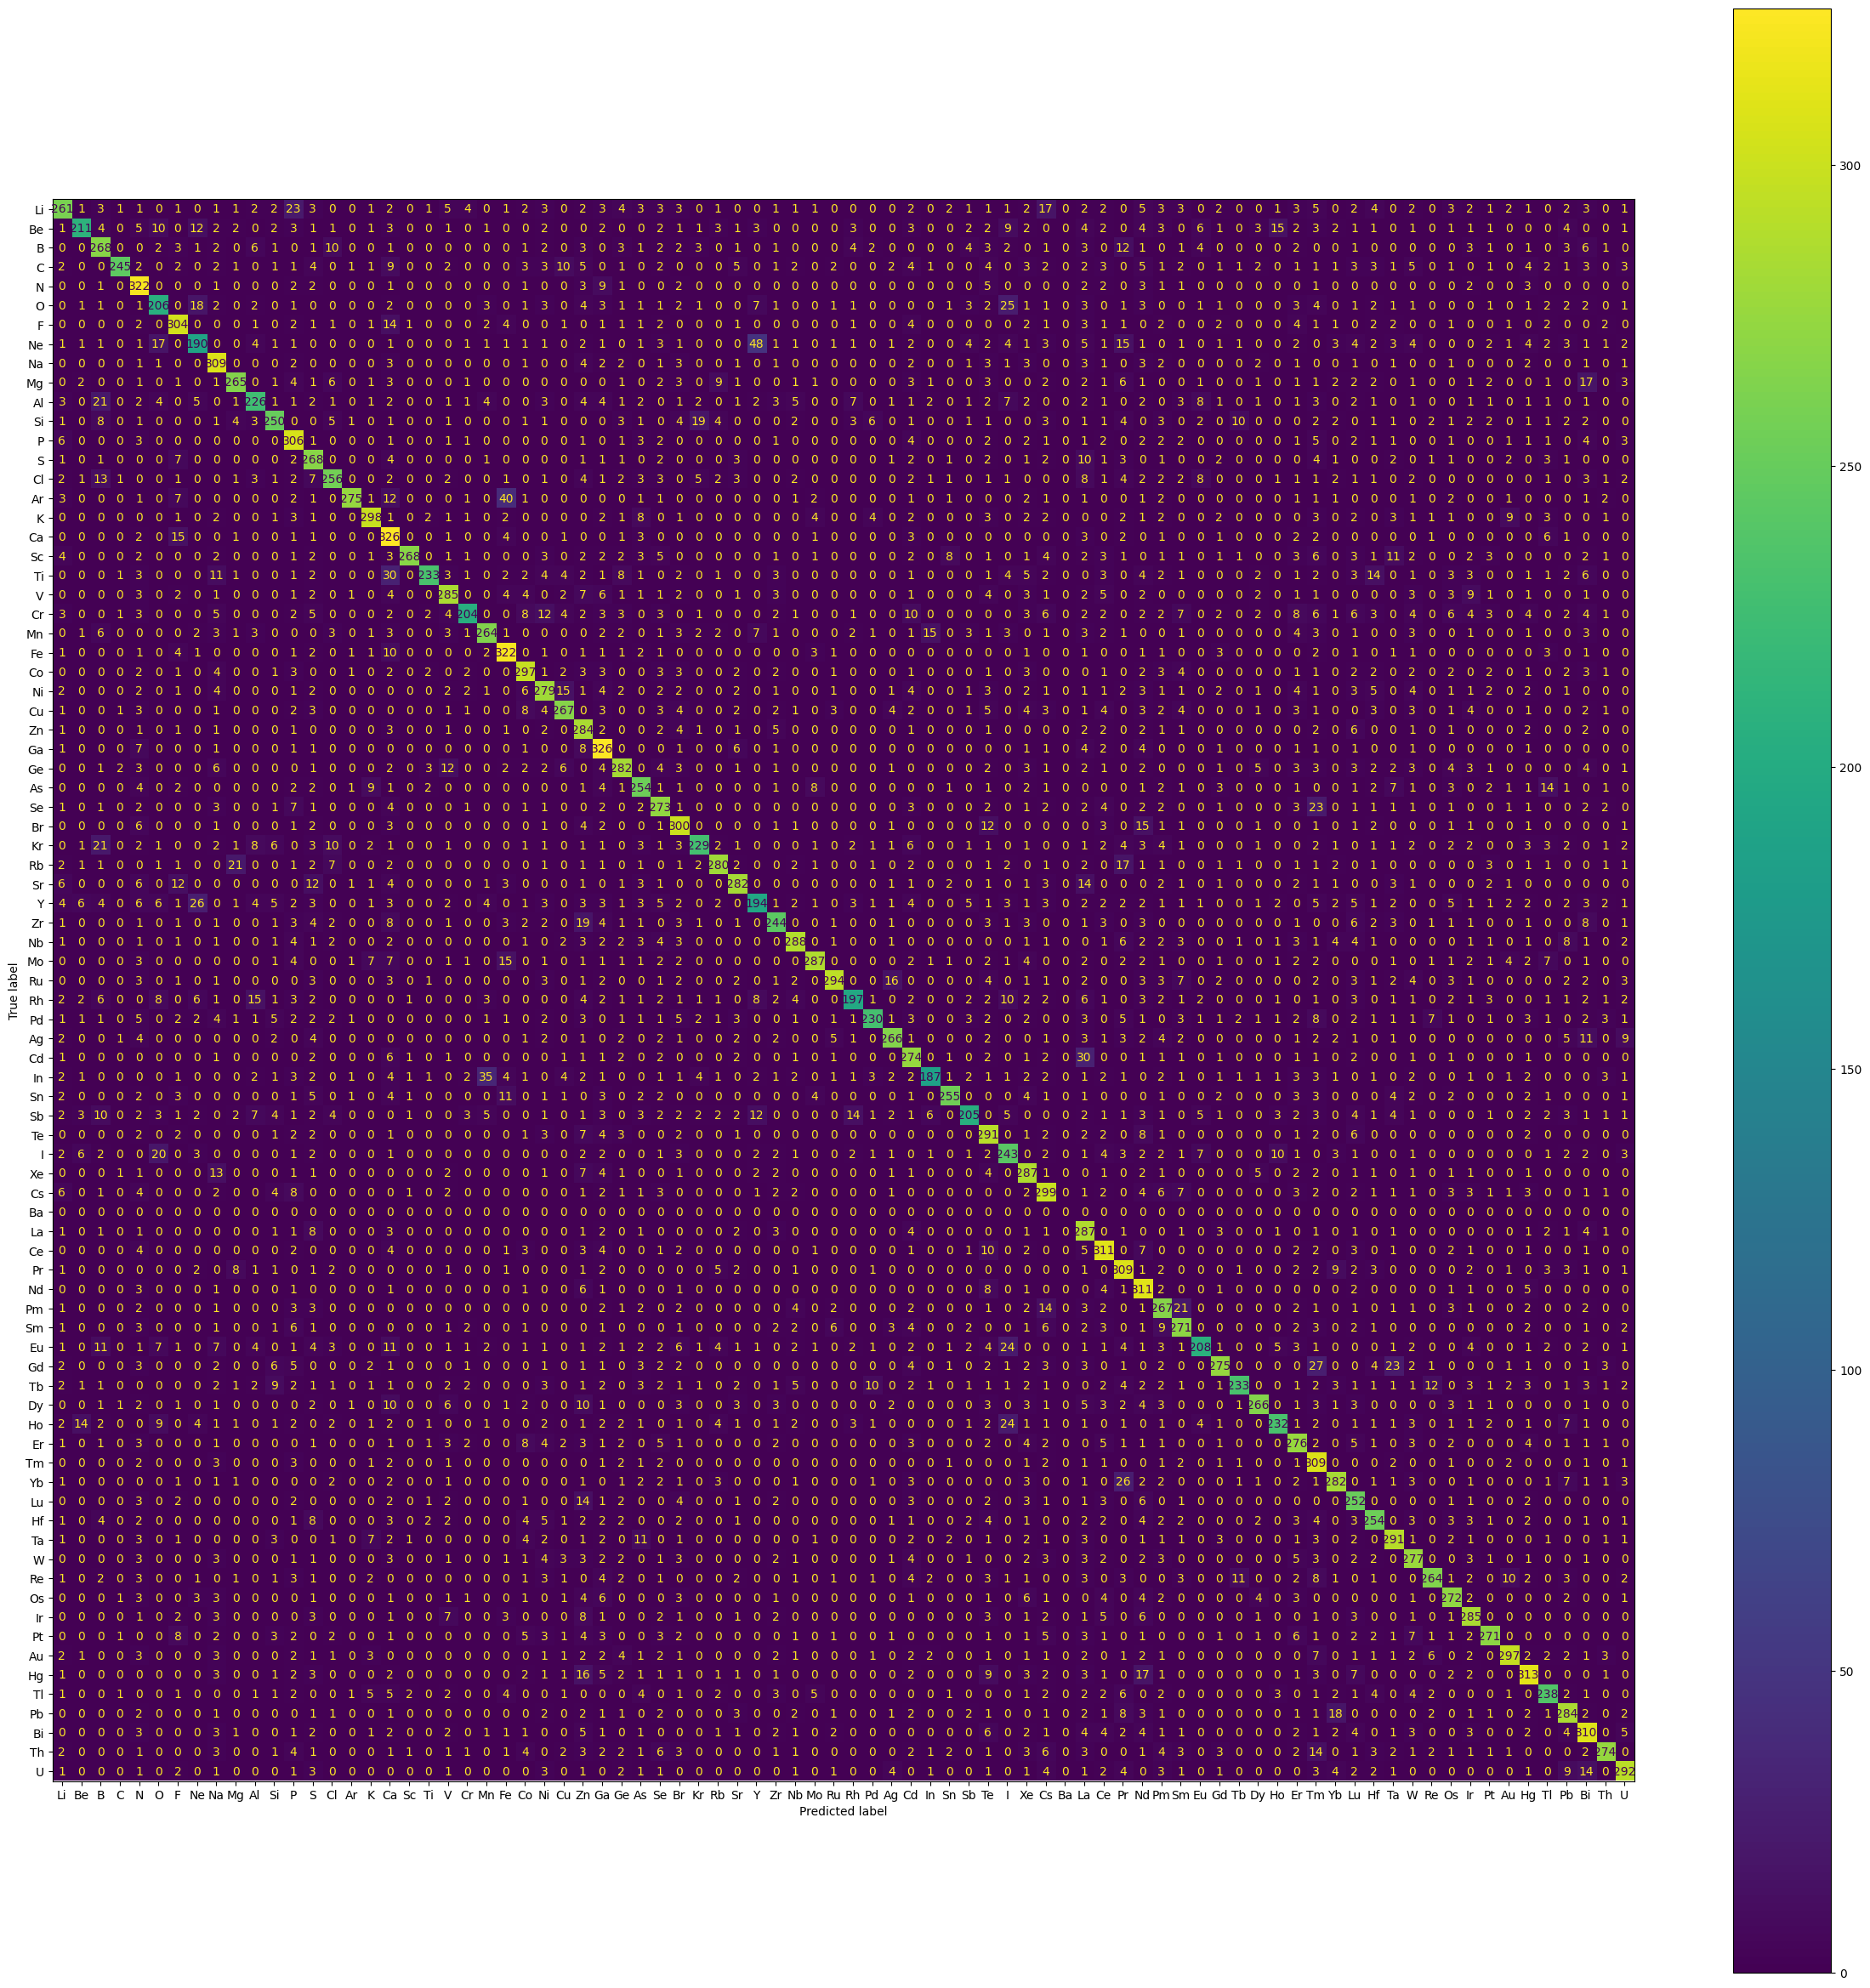
\includegraphics[width=\textwidth]{Figures/CM_CNN_1L.png}
    \centering
    \caption{Confusion Matrix of Test-Data for CNN Top-Layer prediction}
    \label{cm_cnn_1l}
\end{figure}
\end{center}


%\include{Appendices/AppendixC}
% !TEX root = ../main.tex

%----------------------------------------------------------------------------------------
% APPENDIX: DECLARATION OF ORIGINALITY
%----------------------------------------------------------------------------------------

% Include the official "Plagiatserklärung" as a PDF

% Ensure that a TOC entry is create while suppressing the chapter header
\cleardoublepage
\phantomsection
\addtocounter{chapter}{1}
\addcontentsline{toc}{chapter}{\protect\numberline{\thechapter} Declaration of Originality}
% The above replaces this command (which creates a chapter header).
%\chapter{Declaration of Originality} % Main appendix title
\label{DeclarationOfOriginalityZHAW}

% Include a PDF (full page)

\includepdf[pages=-]{Appendices/Declaration of originality Master's Thesis.pdf}
 


%----------------------------------------------------------------------------------------
% BIBLIOGRAPHY
%----------------------------------------------------------------------------------------
\printbibliography[heading=bibintoc]

%----------------------------------------------------------------------------------------

\end{document}  
